\section{Selected Architectural Style and Patterns}
This section clarifies the architectural style and architectural pattern adopted in the design of the DREAM system.
The main difference between the two is that an architectural style is the application design at the highest level of abstraction, it is a name given to a recurrent architectural design; while an architectural pattern is a way to implement an architectural style, it is a way to solve a recurring architectural problem related to it.

\subsection{Architectural Style: Client-Server}
In the design of the DREAM application a three tier architecture has been used. It is a client-server architecture in which the functional process logic, data access, computer data storage and user interface are developed and maintained as independent modules on three levels:
\begin{itemize}
    \item a presentation tier;
    \item a logic tier;
    \item a data tier. 
\end{itemize}

In this type of architecture there is the thin client, that is the device that requests the resource, equipped with a user interface in charge of the presentation-level functions. Then, there is the application server, also called middleware, in charge of providing the resource and communicating with the server database, which stores the data used by the application.

The main advantage of the three-tier architecture is the logical and physical separation of functionality. This allows each tier to run on a separate operating system and server platform that best suit its functional requirements.

Compared to one or two tier architecture, this allows for \textbf{faster development} as each tier can be developed simultaneously by several teams. Furthermore, this separation of levels allows programmers to use the latest and best languages and tools for each level.

Moreover, any tier can be scaled independently of the others as needed and if one tier is interrupted, it will be less likely to impact the availability or performance of the other tiers, so this architecture also has a positive impact on \textbf{scalability} and \textbf{reliability} as well.

Since the presentation layer and the data layer cannot communicate directly, a well-designed application layer can function as a kind of internal firewall, preventing some malicious attacks and ensuring \textbf{greater security}.

\subsection{Architectural Pattern: Model-View-Controller Structure}
DREAM application can be structured with the Model-View-Controller (MVC) pattern.
The MVC structure consists of three building blocks: model, view, and controller.
\begin{itemize}
    \item the \textbf{Model} provides the methods to access the data useful for the application;
    \item the \textbf{View} displays the real user interface for the presentation of the data contained in the model and deals with the interaction with users;
    \item the \textbf{Controller} receives the user's commands through the view and implements them by accessing the Model and defining the corresponding View to be presented
\end{itemize}

\begin{figure}[H]
  \centering
  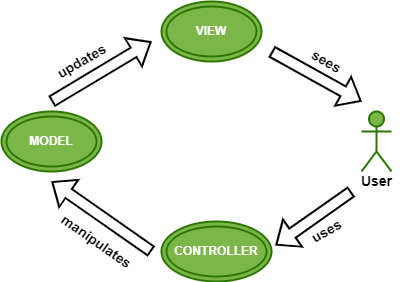
\includegraphics[scale=0.7]{./Images/MVC.png}
  \caption{Model-View-Controller structure}
\end{figure}

This pattern was chosen primarily because application development becomes fast. In fact, it is easier for multiple developers to collaborate and work together given the nature of the architecture itself.
As a result, it also becomes easier to update the application and debug as we have multiple levels properly written in the application.